\documentclass[letterpaper]{article}
%\usepackage{../../../LaTeX/styles/aaai}
\usepackage{aaai}
\usepackage{times}
\usepackage{helvet}
\usepackage{courier}
\usepackage{latexsym} 
\usepackage{graphicx}
\usepackage{algorithm}
\usepackage{algorithmic}

\usepackage{amsmath}
\usepackage{amssymb}

\newtheorem{df}{Definition}
\newtheorem{notation}{Notation}
\newtheorem{theorem}{Theorem}
\newtheorem{lemma}{Lemma}[section]
\newtheorem{col}{Corollary}
\newcommand{\bt}{\begin{theorem}\em}
\newcommand{\et}{\end{theorem}}
\newcommand{\Qed}{$\blacksquare$}
\newcommand{\qed}{$\Box$}
\newcommand{\proof}{{\bf Proof. }}

\newcommand{\nin}{\noindent}

\newcommand{\bea}{\begin{eqnarray}}
\newcommand{\eea}{\end{eqnarray}}

\newcommand{\bdf}{\begin{df}\em}
\newcommand{\edf}{\end{df}}

\newcommand{\ben}{\begin{enumerate}}
\newcommand{\een}{\end{enumerate}}
\newcommand{\ie}{\item}

\newcommand{\dist}{\operatorname{dist}}

\newcommand{\avg}{\operatorname{avg}}


\numberwithin{equation}{section}
\numberwithin{theorem}{section}
\numberwithin{lemma}{section}
\numberwithin{df}{section}

\title{Search Strategies in Multi-Player Drafting Games  \\ \small \vspace{0.1cm} CMPUT 651 Progress Report}

\nocopyright

\author{Neesha Dessai, Richard Gibson \and Richard Zhao \\
Department of Computing Science, University of Alberta \\
Edmonton, Alberta, T6G 2E8, Canada \\
$\{$neesha$\mid$rggibson$\mid$rxzhao$\}$@cs.ualberta.ca}


\begin{document}

\maketitle

\begin{abstract}
A \emph{drafting game} is a game played by a set of $n$ players, where items are picked in turn without replacement from a communal collection.  Players attempt to maximize an individual end-game reward signal based on the unordered sets of choices made by each of the players.  We present two algorithms for playing drafting games, called MaxN-MC and KthBestPick.  (More abstract to come once we finish results).
\end{abstract}

\section{Introduction}

% Talk about search for single agent, minimax for two-player, 0-sum, MaxN for multi-player.  Examples like chess, checkers, etc.

For at least the past few decades, games have been an exceptional platform for artificial intelligence research.  Many successful computer programs have been developed which play at expert levels in two-player games such as Othello, Hex, checkers, chess, and Go.  These games can be handled reasonably well by classic and modern artificial intelligence techniques, such as minimax search and Monte-Carlo tree search.  However, multi-player (i.e., more than 2 players) games are less understood.  In this paper, we explore strategies for playing multi-player ``drafting games.''  Informally, a drafting game involves players taking turns selecting from a collection of items without replacement until some end game condition has been met.  At the conclusion of the game, each player receives an individual reward based on who chose which items; the order of the selections is irrelevant.  The objective for each player is to maximize her individual end game reward.  Some challenges associated with drafting games are dealing with large action spaces, and considering how the choices of other agents should effect our own.

% Also include Risk in this discussion
There are a number of games, including both traditional board games and modern commercial video games, which either can be modeled as a drafting game, or incorporate some kind of draft within part of the game.  Hex is an example of a two-player drafting game, where players take turns picking positions on the board, placing coloured stones on those positions to indicate their selections.  We can consider the player in the winning position at game's end receiving a positive reward, while the losing playing receives nothing.  Another example is a variation of the board game Risk by Hasbro Inc., which begins by players drafting the territories on the board until every territory has an owner.  If we know the strategies which the players will follow for the rest of the Risk game, then we can model the rewards as the likelihoods that each player will win following those strategies, given how the territories were drafted.  As for video games, sports simulations in particular often include a drafting aspect.  For instance, when playing through multiple seasons of the baseball game \textit{MLB 09: The Show} from Sony, a rookie draft takes place in between each season, where the human player and the computer opponents take turns choosing from a pool of new players who may then be added to the respective team's roster.  Another example is the new hockey game \textit{NHL 10} by EA Sports, where a fantasy draft can be activated at the beginning of a season.  In a fantasy draft, all players are removed from their current teams, and then selected one-by-one by the agents (human or computer-controlled teams) in the league.  The rewards at the end of these drafts could be realized by some measure of team improvement or overall team strength, according to the ratings of the players chosen.

% What is our goal/contribution?  When are our algorithms best suited?
This paper contributes two strategies for playing drafting games.  The first, MaxN-MC search, considers all possible actions of all players for a fixed number of turns, and then randomly simulates the remainder of the draft to evaluate those actions.  While designed with drafting games in mind, MaxN-MC can also be used to play other multi-player games.  The second approach, the KthBestPick algorithm, is a drafting-game-only strategy which picks a valuable action, according to some heuristic, that is believed to be sought after by at least one other player.  We use Risk as a testbed for our drafting techniques.

% Outline rest of the paper

Work to be done:
\begin{itemize}
	\item Should we include an outline of the rest of the paper here?
\end{itemize}

\section{Problem Formulation}
\label{sec:Prob}

% Maybe turn this section into Introduction and Background?

We now formally introduce the problem of drafting.  A \emph{drafting game} is a finite, deterministic, full-information game played by a set of $n$ players, which we label 0 through $n-1$.  The game has a single set of actions or \emph{picks} $A$ initially available to every player.  Once a player makes a pick, that pick is forbidden to all players for the rest of the game.  Play continues until some predefined end game condition is satisfied, or all actions in $A$ have been chosen.  At the game's conclusion, the picks made by each of the players induce a partition $Z = \{A_0, A_1, ..., A_{n-1}, \bar{A}\}$ of $A$, where $A_i$ is the set of all picks made by player $i$, and $\bar{A}$ are the actions that were not chosen by any player.  Each player then receives a reward signal $r_i(Z)$ according to the resulting partition $Z$.  Player $i$'s objective is to make picks in such a way as to maximize $r_i(Z)$.

%In many applications, a drafting game is a precursor to a larger competition involving the same set of players.  For example, in Risk, players first participate in a drafting game, taking turns selecting territories until all territories on the map are occupied.  The game then continues until a single player wins by occupying all territories on the map.  When the drafting game is a prelude like this, it is sensible to model the reward signal $r_i(Z)$ as the probability that player $i$ wins the ``larger'' game, given that $Z$ is the result of the draft.  We use this as our reward signal for our experiments with drafting in Risk.

\section{Related Work}

Perhaps the most widely known approach to computer game playing is the minimax adversarial search algorithm.  It is designed for zero sum games involving two players, denoted Max and Min.  The Max player (assumed to be the active player) performs a search of a game tree rooted at the current state of the game.  Each leaf node of the tree is evaluated by a heuristic function, which returns a value estimating the merit of the state to Max.  These values are then backed up the tree; at nodes belonging to Max, the maximum value of all child nodes is propagated up, whereas at nodes belonging to Min, the minimum value of the children is backed up.  The Max player then chooses the action leading to the child with the maximum propagated value.

% MaxN, Paranoid
% MP-Mix which extends MaxN (was used only for branching factor of 3, and for single winner games)

While minimax search is a traditional strategy employed in many two-player games, it is not applicable to games with $n > 2$ players.  Perhaps the simplest generalization of traditional minimax search to more players is the MaxN algorithm \cite{MaxN}.  At the leaf nodes of the game tree, a heuristic function now estimates a vector of $n$ merits $(h_1, ..., h_n)$, one for each player.  At nodes belonging to player $i$, the vector with the highest $h_i$ value is propagated up to the parent.  Thus, players are assumed to be maximizing their own individual payoffs throughout the remainder of the game.  An alternative to MaxN is the Paranoid algorithm \cite{Paranoid}, where the active player assumes that the other players are out to minimize her payoff with complete disregard to their own benefits.  The Paranoid algorithm is essentially equivalent to the minimax algorithm, where the other players are represented as one meta-player (Min) attempting to minimize the individual heuristic value of the active player (Max).  Finally, the MaxN and Paranoid propagation strategies can be dynamically selected according to the game situation.  This is done in the MP-Mix algorithm \cite{ZuckFelnerKraus2009}, along with a third strategy called Offensive.  However, MP-Mix was designed for games with only a single winner, which does not directly fit into the framework of a drafting game.

% Monte Carlo Tree Search in Go
Monte-Carlo tree search algorithms, such as UCT \cite{UCT}, are a different approach to game playing than minimax-type methods.  Simply put, thousands of games are simulated to completion, and each node's value is set to the average of the outcomes which passed through that node.  As game tree sizes typically grow exponentially in their branching factor, minimax-type algorithms must often rely on an accurate heuristic function at non-terminal nodes due to memory or time constraints.  Monte-Carlo tree search, on the other hand, needs no heuristic function and receives an unbiased estimate of the value of each action.  Because of this, UCT is often preferred in games with large action spaces or which lack a quality heuristic function, and has had much success in Computer Go \cite{ComputerGo}.  However, simple Monte-Carlo algorithms use random action selection during the simulations, which often lead to outcomes that will never occur among competent players.  Minimax type algorithms, however, assume players behave in some logical manner.  Our first contribution in this paper, MaxN-MC search, is a hybrid of these two approaches.

% Meta-models for reducing action space

In drafting games, the initial action space is typically large.  Rather than resorting to Monte-Carlo techniques, we can try to reduce the set of actions considered by the players to allow deeper minimax-type searches.  One can automate this action-set selection procedure by using a tool called Genetic Algorithms with Meta-Models (GAMM) \cite{GAMM}.  A simpler approach would be to consider only the most favourable actions according to some heuristic values of the immediate children.  Our second contribution, the KthBestPick algorithm, incorporates this simpler idea into a novel search strategy designed specifically for drafting games.


\section{MaxN-MC Search}

% MaxN-MC search

The MaxN-MC algorithm is an adversarial search algorithm for multi-player games.  It applies MaxN search to a fixed depth in the game tree.  Then, at each leaf in the search tree, we do not use a heuristic function to estimate its value as in the regular MaxN algorithm.  Instead, we carry out Monte-Carlo simulations and average the outcomes to evaluate the leaf node.  These outcomes are then what is propagated back to the root of the search in the remainder of the MaxN algorithm.  

\begin{algorithm}[htb]
	\caption{MaxN-MC($node$, $d$, $M$)}
	\label{alg:MaxN-MC}
	\begin{algorithmic}[1]
		\IF{$node$ is terminal}
			\RETURN{payouts associated with $node$}
		\ENDIF
		\IF{$d > 0$}
			\FORALL{$child$ of $node$}
				\STATE $child.value$ $\gets$ MaxN-MC($child$, $d - 1$, $M$)
			\ENDFOR
			\STATE $p \gets node$.getActivePlayer()
			\STATE $bestChild \gets \arg \max_{child \text{ of } node} child.value_p$
			\RETURN{$bestChild.value$}
		\ELSIF{$d = 0$}
			\FOR{$i$ from $1$ to $M$}
				\STATE Pick $child$ of $node$ at random
				\STATE $values(i) \gets $ MaxN-MC($child$, $d-1$, $M$)
			\ENDFOR
			\RETURN{component-wise average of $values$}
		\ELSE
			\STATE Pick $child$ of $node$ at random
			\RETURN{MaxN-MC($child$, $d-1$, $M$)}
		\ENDIF
	\end{algorithmic}
\end{algorithm}

The pseudocode for MaxN-MC is presented in Algorithm \ref{alg:MaxN-MC}.  It receives the current state $node$ of the game as input, as well as two numbers, $d$ and $M$, which denote the depth of the MaxN search and the number of Monte-Carlo simulations to perform at each leaf node respectively.  First, MaxN-MC checks if the game is over (line 1), in which case it returns the associated payouts each player receives (line 2).  For drafting games, we would return the vector of rewards $(r_1(Z), ..., r_n(Z))$, where $Z$ is the partition of the initial action space as described previously.  At a node at depth less than $d$, we make recursive calls on each of its children in the game tree, counting down the depth in the tree on each pass (line 6).  Each call returns a vector of values, one for each player, indicating the merit of the child state to each of the players.  The parent node then finds the child with the best merit for the active player (line 9), and back-propagates this child's vector of values (line 10).  Once we reach a node at depth $d$, we perform $M$ random walks down the game tree, each being initiated by lines 13 and 14, and continued by lines 18 and 19 until reaching a terminal state at line 1.  Finally, for each player, we average the $M$ merits associated with the outcomes of the random walks, and propagate back these averages (line 16).

In drafting games, often the picks made at the beginning of the draft have more of an effect on the outcome than picks near the end of the draft.  For instance, in sports drafts, typically the most valuable players on a team are picked in the first few rounds, while the final picks usually involve weaker players that may only improve the team's overall strength slightly.  This is the motivating idea behind the MaxN-MC algorithm.  First, we consider all ways that the next $d$ picks of the game can play out.  After $d$ picks, we hope that the following picks are less important, and simply simulate random picks to evaluate the position.

Work to be done here:
\begin{itemize}
	\item During game play, we should consider time constraints when making a move.  In drafting games, both the depth parameter $d$ and the number of random simulations $M$ can be dynamically chosen based on the number of total picks remaining in the game in order to achieve real-time play.  Currently, we choose $d$ based on a maximum number of nodes we are willing to expand in the MaxN search.  The same should be done for $M$.
	\item Near the beginning of a draft, there will be a lot of picks available.  So, if we are considering time constraints, this means that typically the depth $d$ that we can search to will be small.  In this case, we should probably increase $M$ to get a ``better'' estimate of the value of the current state.  However, this in turn again increases the time required by the algorithm to run.  What should we do here?
	\item Should we walk through an example using MaxN-MC, or is the algorithm clear enough as is?
\end{itemize}

 
\section{The KthBestPick Algorithm}
% kthBestPick search

While the MaxN-MC algorithm could be applied to any multi-player game, our next contribution, the KthBestPick algorithm, focuses specifically on drafting games.  The idea here is that it may not always be best to pick the action which improves our situation the most.  For instance, suppose we are considering two particular actions, A and B, that we feel will both benefit our end-game reward.  Suppose further that we believe picking A will be slightly more beneficial to us than picking B.  If no other player will benefit themselves from picking A, but a player will benefit from picking B, then we should consider picking B now with our current action, as it seems likely that A will be available with our next pick.  If we choose A now, B may not be available on our next turn.  At each turn, KthBestPick uses a heuristic function to rank the available picks from best (rank 0) to worst (rank equal to the number of picks remaining minus 1).  Then, it estimates the most inferior pick of rank $k$ that we may choose so that we eventually pick all $k$ better-ranked actions (rank 0, 1, ..., $k-1$) with our later picks.  This is done using opponent models to predict the play of the other players.

\begin{algorithm}
	\caption{KthBestPick($node$, $h$, $m_0$, ..., $m_{n-1}$)}
	\label{alg:kth}
	\begin{algorithmic}[1]
		\STATE $rankedPicks \gets $ sort($node$.getActions(), $h$)
		\STATE $p \gets node$.getActivePlayer()
		\FOR{$k$ from $node$.getNumPicksLeft(p)$-1$ to $0$}
			\STATE $pick \gets rankedPicks(k)$
			\STATE $betterPicks \gets rankedPicks(0..k-1)$
			\STATE $child \gets node.$getChild($pick$)
			\STATE $makeThisPick \gets $ TRUE
			\WHILE{$betterPicks$ is not empty}
				\STATE $p \gets child$.getActivePlayer()
				\STATE $nextPick \gets m_p(child)$
				\STATE $child \gets child.$getChild($nextPick$)
				\IF{$nextPick \in betterPicks$}
					\IF{$p = node$.getActivePlayer()}
						\STATE $betterPicks.$remove($nextPick$)
					\ELSE
						\STATE $makeThisPick \gets $ FALSE
						\STATE break
					\ENDIF
				\ENDIF
			\ENDWHILE
			\IF{$makeThisPick$}
				\RETURN{$pick$}
			\ENDIF
		\ENDFOR
	\end{algorithmic}
\end{algorithm}

Algorithm \ref{alg:kth} gives the pseudocode for KthBestPick, which takes in the current state $node$, a heuristic function $h$, and a sequence of opponent models $m_0, ..., m_{n-1}$ (one for each player) as parameters.  We first rank the actions according to the heuristic function (line 1), which is assumed to only considers the merit of the picks in the active player's perspective.  Next, $k$ is set to one less than the number of picks remaining for the active player (line 3), as we do not have enough picks to consider more inferior actions.  Then, we set our potential pick to the action ranked $k$ (line 4), construct a list containing all of the superior picks (line 5), and initialize $child$ to point to the child node associated with this potential pick.  To determine if this pick is desired, we iteratively find each of the next picks made by the players according to the appropriate opponent model (line 10), which returns the action believed to be picked by the active player at the passed in node.  After updating our $child$ pointer to follow this next pick (line 11), we check if the pick is in our list of superior actions (line 12).  If it is, there are two possible cases.  If the pick was taken by the original active player (i.e., the player whose turn it is upon calling KthBestPick) (line 13), then this is allowed; we remove the pick from the superior list (line 14) and continue.  However, if the pick was taken by a player other than the original player, then we abandon our potential pick (lines 16 and 17), decrement $k$ (line 3), and now consider the new potential pick ranked $k$ (line 4 again).  During the iterations, if the list of superior picks ever becomes empty (line 8), this indicates that the original active player is predicted to pick all of the superior actions, and so we return the current potential pick (line 22).

% Possible heuristic functions: learn one based on a number of features describing the current state-action space, or can use MaxN-MC.
There are a number of different possibilities for the heuristic function.  These include using expert knowledge (if available), attempting to learn an evaluator using machine learning techniques, or applying reinforcement learning through self-play.  In either learning scenario, domain-specific features will need to be identified based on the set of picks already chosen by each of the players.  Additionally, one could base a heuristic function on the output of a MaxN-MC call.

% Possible opponent models: KthBestPick (in practice, keep track of repeated calls in one state, and truncate the game to a fixed maximum number of picks remaining), if repeated games then could try to learn an opponent model.  Typically will not be given the explicit opponent drafting strategies.
As for the opponent models, again there are a few options.  Firstly, we should use KthBestPick as the opponent model for our own play, since we know this is the strategy being used to make our picks.  Typically for the other players, however, we will not be given their explicit drafting strategies.  The simplest approach would be to assume that the opponents are also using KthBestPick to make decisions with an appropriate self-centered heuristic function.  This turns line 10 of Algorithm \ref{alg:kth} into a recursive call, and in this case, KthBestPick can be very costly in computation time.  We can combat this in two ways.  First, we can keep track of the calls to KthBestPick and store the results to prevent repeated computations.  Secondly, rather than starting $k$ at the number of picks remaining for the active player, we can shorten the computation time by only considering a fixed number of the highest ranked picks.  Finally, if we play repeated matches against the same opponents, we could learn an opponent model, again using either machine learning techniques or reinforcement learning.

% How to handle tie-breaks?  Should we include a small example and walk through it with KthBestPick?
Work still to be done:
\begin{itemize}
	\item How should we handle tie-breaks in the rankings?  A tie can occur at both line 1 and line 10 (depending on the opponent model).  In the case of a tie in the rankedPicks list, we may want to consider more potential picks than just the number of remaining picks.
	\item Should we walk through a small example?
\end{itemize}

\section{Theoretical Analysis}

\begin{itemize}
	\item Can we show that MaxN-MC converges to a Nash equilibrium, much like MaxN does?  Note that UCT converges to the minimax value (in the two-player case I assume?).
	\item What can be said theoretically about KthBestPick?  Are there conditions on the heuristic function and/or the opponent models which make KthBestPick an ``optimal'' strategy in some sense?
\end{itemize}

\section{Empirical Evaluation}

All of our experiments will be conducted in the board game Risk using the Lux Delux\footnote{http://sillysoft.net/lux/} environment.  Lux Delux provides several Risk bots with source code, which include their own hand-coded drafting strategies.  Conveniently, this gives us plenty of competition to test our algorithms against.  We use the selected countries and even initial army placement options in all of our experiments.

An evaluation function in Risk is provided by (Johansson & Olsson 2006), and in more detail in (Olsson 2005), to calculate the value of a single territory.  This territory value is meant to approximate how desirable an enemy territory is to a player during gameplay.  The evaluation function is a sum of different sub-components, each measuring a unique situation in the game.  Advantageous situations are given positive values and disadvantageous situations are given negative values.  For example, it is desirable to have more friendly neighbours around a territory, thus the number of friendly neighbours to a territory is a sub-component that contribute positively to the value of this territory.
We adopted this evaluation function to measure the value of an entire draft to a particular player.  The territory values given by the evaluation function for all territories owned by the player are added together, creating a draft evaluation function.  However, we have to make changes to Johansson & Olsson’s territory evaluation function (from here on referred to as JO) since some sub-components are not longer valid with our new intended purpose:
\begin{itemize}
JO gives a value of 0.05 for each army in a friendly neighbour and -0.03 for each army in an enemy neighbour.  Since we are evaluating a complete draft before the post-draft play (where the placing of armies occur), these two components do not apply to us.
JO gives a value of 20 for owning the whole continent except this territory.  Thus this territory has a high value to the player.  Such a territory is highly desirable since obtaining an entire continent provides a bonus to armies.  In our case, we only give the same value for actually owning the whole continent, since in a final draft all territory ownerships are determined.
JO gives a value of 4 if an enemy owns the whole continent. In such cases, conquering this enemy territory is desirable since it prevents the enemy from getting the continent army bonus.  In our case, if an enemy owns a continent in the final draft, then it is disadvantageous for the player, so a value of -4 is given.
\end{itemize}	
	

\subsection{Analyzing Evaluation Function}

Before we committed to using the new evaluation function as we modified from the paper, we needed to test how well it worked at predicting completed draft states. To test this, we created 6 random draft configurations. These were created by having three agents randomly pick a territory, and then storing the values chosen by each so that they could be recreated later. Therefore, each draft configuration was made up of three sets of draft picks, one for each of the three players (agents). An example map is shown in Figure~\ref{fig:random}. We had a 7th draft configuration where one agent owns an entire continent, in this case Australia, which is shown in Figure~\ref{fig:continent}. 

Next, we computed the evaluation function for each set of picks in each draft. From there, each draft was used to play two sets of 1000 games. The first 1000 games were played such that each agent chose their draft picks based on their turn order, so whichever agent went first on each game chose from set 0. The second set of 1000 games were played such that each agent always choose the same draft picks regardless of order, ie one agent always choose from set 0, one from set 1 and the third from set 2. The number of games each set won for each draft are presented in Table~\ref{tab:results}.

The results show that there are draft combinations that the evaluation function is not taking advantage of, as show in the results for player 2 in set 1, or player 0 in set 2. The other interesting result is that for some draft selections, being the first player (as shown in the ordered results) can be an advantage, something we expected. But, there are cases where a draft set actually does better in the random configuration. By running more tests of the 6 possible orders for the three agents, we may be able to learn more about the advantages/disadvantages the turn order provides. 

\begin{figure}[htp]
\centering
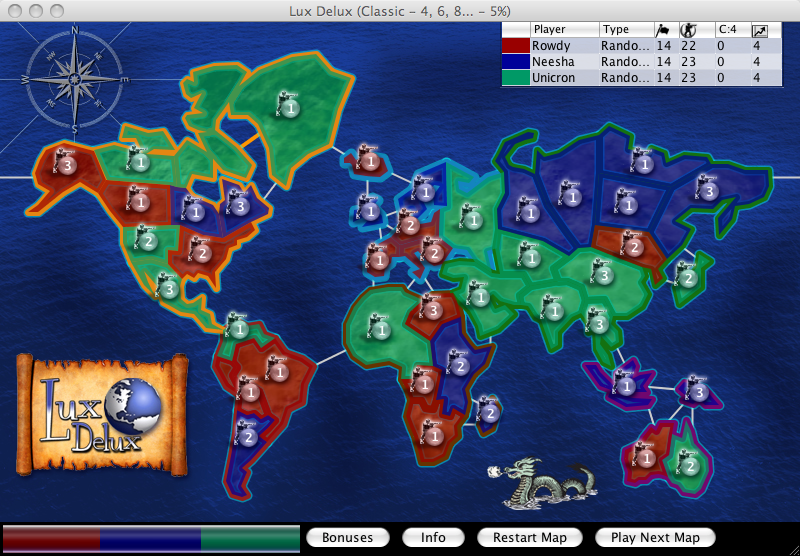
\includegraphics[scale=0.3]{testmap2.png}
\caption{Example random draft selection.}\label{fig:random}
\end{figure}

\begin{figure}[htp]
\centering
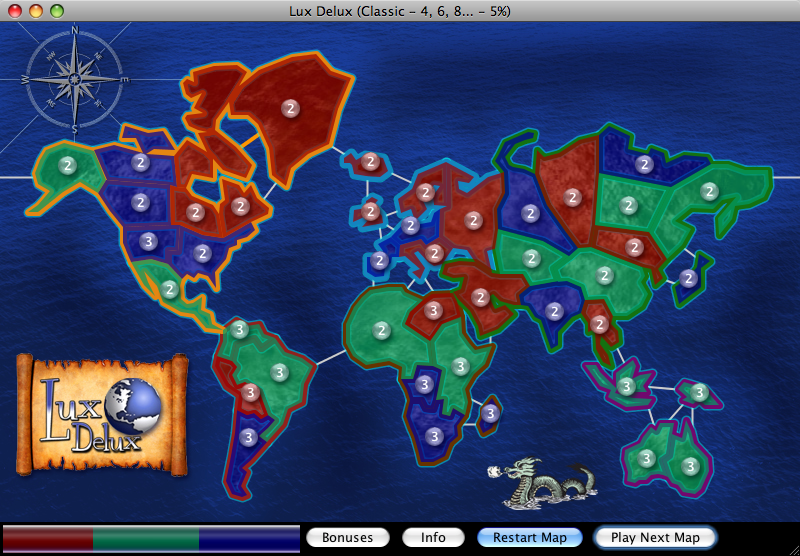
\includegraphics[scale=0.3]{testmapcontinent.png}
\caption{Draft selection so that a single player owns a whole continent.}\label{fig:continent}
\end{figure}

\begin{table}[]
%\begin{center}
%\centering      % used for centering table 
\begin{tabular}{l l r r r}  % centered columns (5 columns) 
\hline                       %inserts double horizontal lines
Draft &  & 0 & 1 & 2 \\[0.5ex]% inserts
\hline                    % inserts single horizontal line
0&Evaluation Function&0.278&0.345&0.377\\
&Ordered&283&360&357\\
&Unordered&420&304&276\\
1&Evaluation Function&0.317&0.343&0.34\\
&Ordered&322&272&406\\
&Unordered&258&309&433\\
2&Evaluation Function&0.347&0.342&0.312\\
&Ordered&412&354&234\\
&Unordered&373&342&285\\
3&Evaluation Function&0.323&0.361&0.306\\
&Ordered&293&368&339\\
&Unordered&347&287&366\\
4&Evaluation Function&0.288&0.333&0.379\\
&Ordered&330&374&296\\
&Unordered&356&368&276\\
5&Evaluation Function&0.362&0.302&0.336\\
&Ordered&405&356&239\\
&Unordered&317&332&351\\
6&Evaluation Function&0.195&0.231&0.573\\
&Ordered&216&271&513\\
&Unordered&247&199&554\\
[1ex]
\hline     %inserts single line 
\end{tabular} 
%\label{table:nonlin}  % is used to refer this table in the text 
%\end{center}
\caption{\label{tab:results} Results of evaluation function and sets on the draft configurations..}
\end{table}


\subsection{Evaluating MaxN-MC using Evaluation Function}

We have run experiments to get an idea of the effectiveness of MaxN-MC using our new evaluation function.  The experiments are set up to have three players.  All three players have identical post-draft strategies provided by a hard-coded Lux agent (namely EvilPixie).  The difference is in the strategies employed in the drafting stage.  While Players 1 and 2 use the hard-coded rules of EvilPixie, Player 0 uses MaxN-MC with our new evaluation function.  Six sets of experiments were run on the world map, each set consisting of  $ to # episodes.  An episode is defined as a complete game where each player used their own strategy in the drafting stage then played until a winner is emerged.  
The results are presented in Table~\ref{tab:experiments}.  MAX_NODES represents the depth in MaxN search where Monte Carlo roll outs take over. NUM_ ROLL_OUTS represents the number of Monte Carlo roll outs that we average over in MaxN-MC, for each leaf node of the MaxN portion of the search.  A different number of episodes were run for each set of experiments because we have constrained each set to a 24-hour period, and having a larger MAX_NODES or a larger NUM_ ROLL_OUTS means that each episode will take longer time.  All experiments show promising results that Player 0 has won a higher number of episodes than the other two players.  Because these results are still preliminary, no conclusions can yet be made.

\begin{table}[]
%\begin{center}
%\centering      % used for centering table 
\begin{tabular}{r r r r r r}  % centered columns (6 columns) 
\hline                       %inserts double horizontal lines
MAX_NODES & NUM_ ROLL_OUTS & Total episodes & Player 0 winning rate & Player 1 winning rate & Player 2 winning rate \\[0.5ex]% inserts
\hline                    % inserts single horizontal line
1000&10&190&0.468&0.274&0.258\\
5000&10&216&0.384&0.361&0.255\\
10000&10&134&0.425&0.291&0.284\\
100&100&241&0.432&0.266&0.303\\
500&100&156&0.423&0.346&0.231\\
1000&100&63&0.460&0.206&0.333\\
[1ex]
\hline     %inserts single line 
\end{tabular} 
%\label{table:nonlin}  % is used to refer this table in the text 
%\end{center}
\caption{\label{tab:experiments} Results of experiments comparing drafting strategies of MaxN-MC with EvilPixie}
\end{table}

\subsection{Work still to be done:}

\begin{itemize}
	\item Build a heuristic function for the KthBestPick algorithm using RL.
	\item Run experiments for the KthBestPick algorithm.  Compare the heuristics: MaxN-MC, RL (see above point), and perhaps some further modification of the evaluation function in \cite{RiskBots}.
	\item Since we have the opponent drafting strategies, maybe try running KthBestPick with these ``oracle'' opponent models, versus simply using KthBestPick as the opponent models.
	\item Note that it is important that the drafting strategy plays well with the post-draft strategy.  For instance, if our post-draft strategy is to conquer Europe but we claim South America in the draft, then this overall strategy is likely to perform very poorly (compared to a post-draft strategy which tries to keep South America).  This indicates that a learning technique incorporating post-draft performance may be better suited than expert-knowledge.
	\item We plan to report our results in much the same manner as in \cite{ZuckFelnerKraus2009}.
\end{itemize} 


\section{Conclusions}

% Summarize what we have so far with the algorithms and empirical results

This paper has formalized the concept of a drafting game.  As the action spaces are large and the actions of multiple opponents must be considered, traditional game playing strategies are not directly applicable.  We introduced two solutions for playing a drafting game.  Our first approach, MaxN-MC, is a combination of the MaxN algorithm, which generalizes minimax search to multi-player games, and Monte-Carlo simulations, as used in Monte-Carlo tree search algorithms.  Our second technique is KthBestPick, which uses heuristics to rank actions and opponent models to predict which actions will be selected by other players.  

Work to be done:
\begin{itemize}
	\item Include details of the experimental results to be run, and discuss the strengths (and possibly weaknesses) of the two approaches.
\end{itemize}

We conclude by listing some possible avenues of further research:
\begin{itemize}
	\item using path refinement and abstraction in the space of actions, particularly for MaxN-MC.  In Risk, the 42 territories are naturally grouped into 6 continents.  We could replace the actions from picking territories to picking continents (where each continent is represented a number of times equal to the number of territories in that continent), which would reduce the total search space.  If we can evaluate picks according to just continents, then we could find a path of picks in continent space and then search this corridor in territory space.
	\item restricting the branching factor in MaxN-MC using a territory heuristic like in KthBestPick.
	\item using automated feature selection for developing the heuristic function of KthBestPick, and for estimating the reward signal in MaxN-MC.
\end{itemize}

%\section*{Acknowledgments}
%
%

%\bibliography{../../../LaTeX/bib}
%\bibliographystyle{../../../LaTeX/Styles/aaai}
\bibliography{bib}
\bibliographystyle{aaai}

\end{document}
